\documentclass{article}
\usepackage{geometry}
\usepackage{enumitem}
\usepackage{parskip}
\geometry{
	a4paper,
	total={210mm,297mm},
	left=25mm,
	right=25mm,
	top=25mm,
	bottom=25mm
}
\setlist[description]{leftmargin=\parindent,labelindent=\parindent}
\usepackage[utf8]{inputenc}
\usepackage{graphicx}
\graphicspath{{Bilder/}}

\renewcommand{\contentsname}{Inhaltsverzeichnis}
\begin{document}

\pagenumbering{roman}

\title{Software Projekt - Excel als SQL Datenbank}
\author{Authoren: Rijad \v{Z}u\v{z}o , Séverin Müller \\ \\ Dozent: Ulrich Hauser}

\maketitle

\vspace{80mm}
\begin{center}
		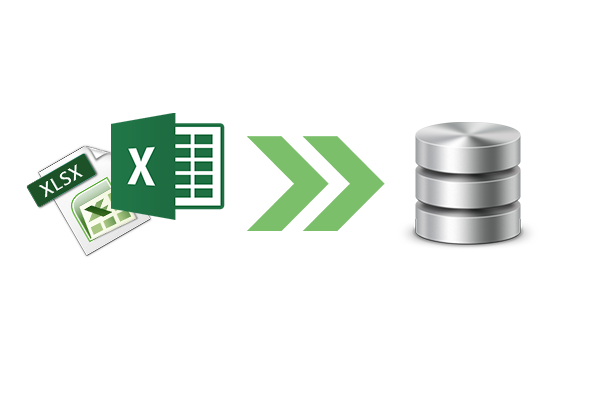
\includegraphics{SoftwareLogo}
\end{center}

\newpage
\tableofcontents
\newpage

\pagenumbering{arabic}

\section{Motivation}
Die Motivation für dieses Projekt stand aus dem Beruflichen Leben. Ein Excel File das zum einfachen auflisten einiger Daten erstellt wurde, kann schnell in eine richtige Datenbank auswachsen.

\subsection{Ausgangssituation}
Das auslesen eines größeren Excel Files ist deutlich langsamer als einer normalen SQL Datenbank der gleichen grösse, deshalb ist es sinnvoll das Excel File in eine SQL Tabelle umzuwandeln. \newline 
Die Konversion erfordert zusätzliche Software Kenntnisse die in dieser Situation unwahrscheinlich sind. \\

Mit der x2dB Applikation wurde das Problem gelöst. Die Umwandlung ist unnötig und somit kann das Excel File bestehend bleiben.

\subsection{Lösungsidee}
Die Idee ist es jetzt eine Applikation mit simplem User-Interface zu entwickeln, welches im Hintergrund das Excel File wie eine SQL Tabelle behandelt und sich über entsprechende Treiber mit dem File verbindet. Das ermöglichen uns die Microsoft.Office.Core und Microsoft.Office.Excel.Interop Treiber. \\

Durch das benutzen der Applikation hat der User einen begrenzten Einfluss auf das File, welches die Kollision bei zbsp. einem Shared File vermeidet. Die Verbindung dauert nur so lange bis die Daten gelesen/geschrieben wurden und danach wird das File wieder freigestellt.

Für zusätzliche Datensicherheit wird nach entsprechender Zeit ein Backup File erstellt und einsetzbar sein. Dies ist natürlich nicht eine Endlösung aber eine guter fix für solche problematische Legacy Situationen.

\section{Anforderungsliste}
Für die Applikation stellen sich jetzt gewisse Anforderungen- Da es sich um eventuell sehr wichtige Daten handelt, darf es in diesem Prozess keine Datenverluste und ähnliche Ausfälle geben. 
	
\subsection{Muss-Anforderungen}
Die Applikation muss:
	\begin{description}
		\item[M1:] Verbindung zum Excel File erstellen.
		\item[M2:] Aus dem File Auslesen und Einschrieben können.
		\item[M3:] Nach dem Auslesen und Einschreiben die Verbindung trennen.
		\item[M4:] Nach gewisser Zeit einen  Backup erstellen.
	\end{description}

\subsection{Soll-Anforderung}
Die Applikation soll:
\begin{description}
	\item[S1:] Leicht Bedienbar sein.
	\item[S2:] Ein angenehmes User-Interface haben.
	\item[S3:] Den User vom Excel File abgrenzen.
\end{description}

\subsection{Wunsch-Anforderung}
Die Applikation könnte:
\begin{description}
	\item[W1:] Eine Benutzungsanleitung haben.
	\item[W2:] Mehrere Sprachen unterstützen.
\end{description}

\newpage

\section{Projektumgebung}
\vspace{5mm}
\subsection{Entwicklungsprozess	}
Da es sich um eine Applikation handelt welche eng mit dem User verbunden ist kann es auch //TODO SCRUM

\subsection{Programmiersprache}
Die Excel Software lauft ausschließlich auf Microsoft Windows Betriebssystemen, deshalb haben wir uns für die Windows Spezifische Programmiersprache C\# entschieden. \\ Diese in Kombination mit der IDE Visual Studio ermöglichten uns eine angenehme Entwicklung sowohl der Funktionalität und auch des GUI's.
 

\subsection{Verwaltungssystem}
Die Auswahl des Verwaltungssystem war sehr einfach da wir die Software als Open Source ausgeben wollten. Wir haben uns für das Git System entschieden und hosteten unser code auf der Website GitHub.

\newpage

\section{Projekt Planung}
\subsection{Product Backlog}
\subsection{Sprints}
\subsection{Sprint Stand-up Meetings}
\subsection{Sprint Review}

\newpage

\section{Ablauf der Entwicklung}

\subsection{Modellierung}
Die erste Phase der Entwicklung war das Strukturieren der Software. Wir wollten ein klares Design haben das uns die Weiterentwicklung in der Zukunft ermöglicht. 

\subsubsection{Klassen Diagramm}
\begin{center}
	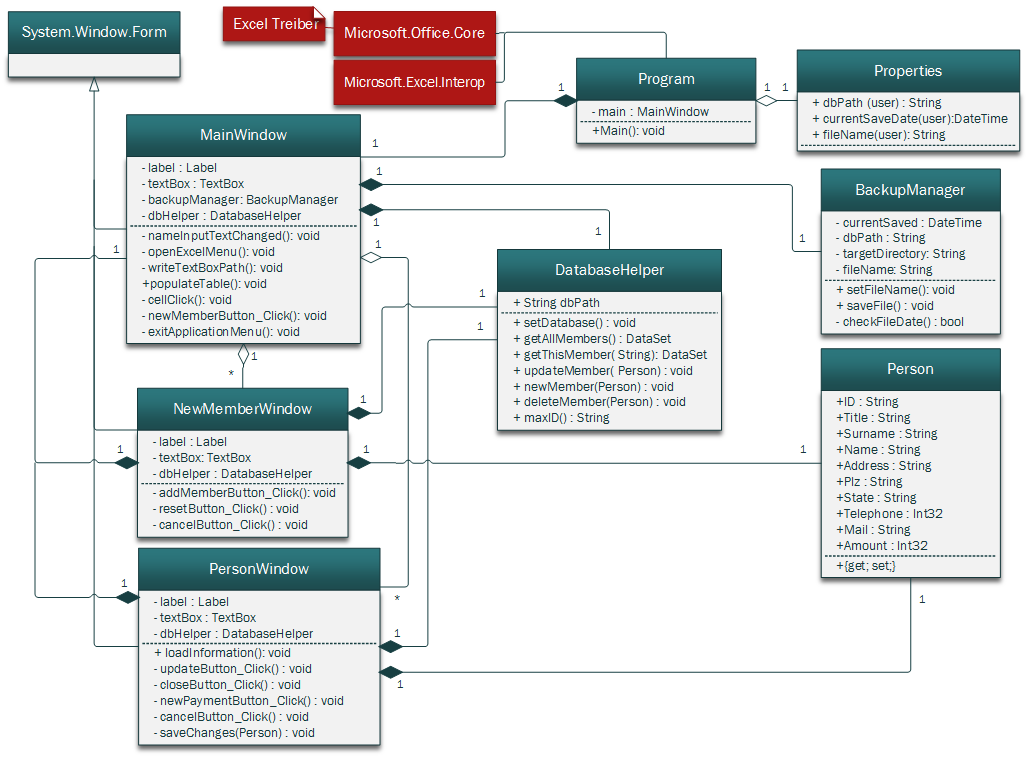
\includegraphics[width=1.05 \textwidth]{KlassendiagrammBild}
	\caption{1.a Klassendiagramm}
\end{center}

\subsubsection{Aktivitäts-Diagramm}

\subsubsection{Sequenz Diagramm}

\subsection{Stunden Journal}
Bild oder tabelle rekreiren von der Stunden template vom Sevi.

\subsection{GUI}
Vorgang bei Gestaltung des GUI's, bedenken usw.

\subsection{Database Handling}
Schwierigkeiten bei den Referenzen, Voraussetzungen zur Verbindung usw.

\subsection{Backup Management}
Ansätze für ein effizientes Backuping :).

\subsection{Testen}
Wie beim Testen vorgegangen wurde!

\newpage

\section{Ziel}
\subsection{Resultat}


\end{document}